\chapter{Experimental Evaluation}
\label{chap:results}

The account of the research should be presented in a manner suitable for the field. It should be complete, systematic, and sufficiently detailed to enable a reader to understand how the data were gathered and how to apply similar methods in another study. Notation and formatting must be consistent throughout the thesis, including units of measure, abbreviations, and the numbering scheme for tables, figures, footnotes, and citations. One or more chapters may consist of material published (or submitted for publication) elsewhere. See “Including Published Material in a Thesis or Dissertation” for details.

\section{Network Implementation Results}

\section{Pruning Algorithm Results}

\section{Terrain Processing Results}

\subsection{Gathered Data} \label{ssec:gathered_data}

\subsubsection*{Data by Sensors} \label{sssec:data_by_sensors}

\begin{figure}[H]
  \centering
  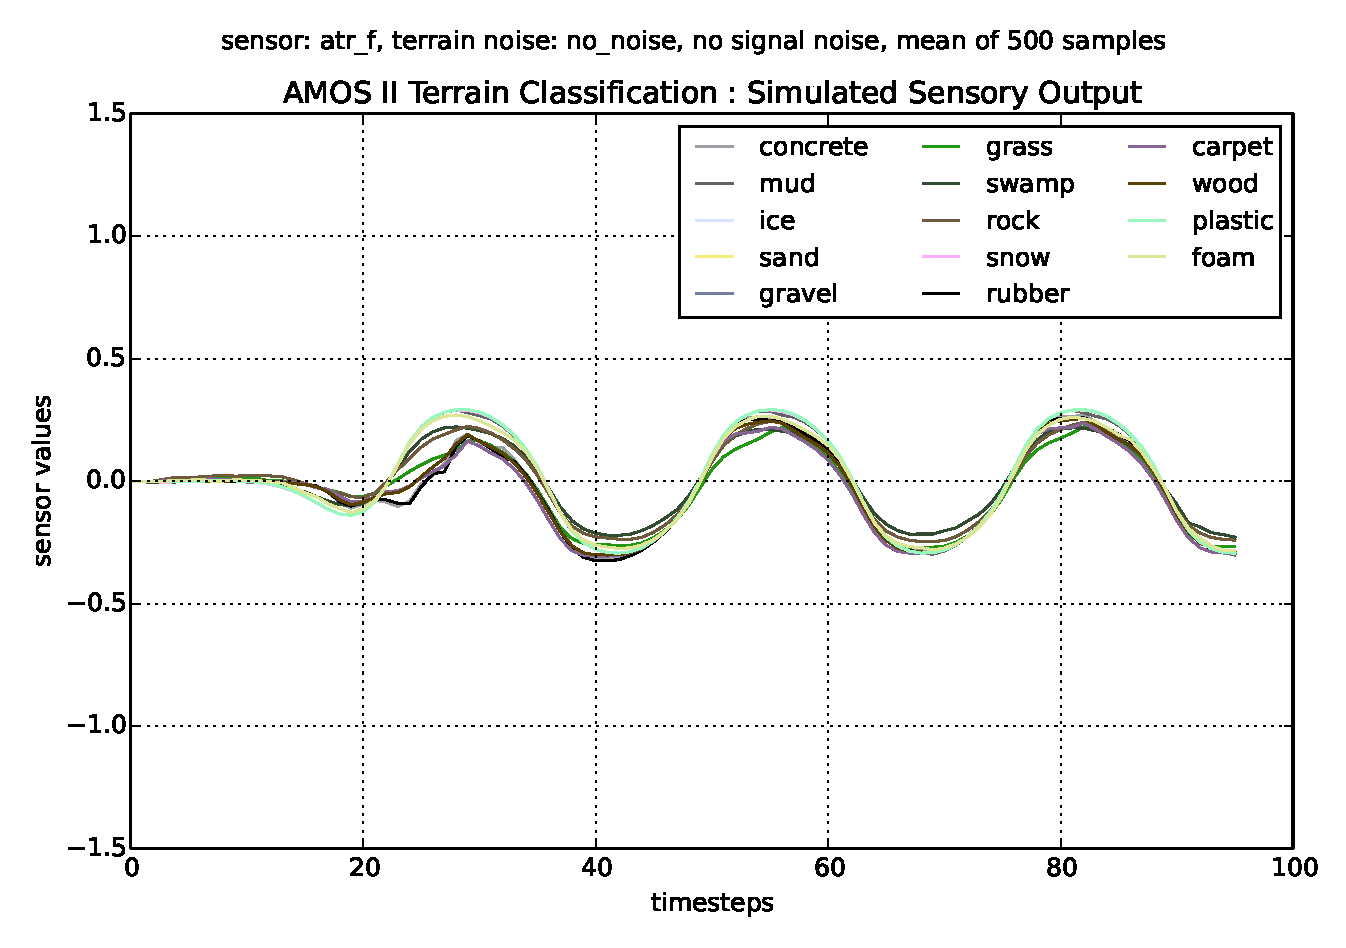
\includegraphics[width=1.0\textwidth]{sensor_atr_f_no_noise}
  \caption{Sensor ATRf : mean of 500 samples, 14 terrains}
  \label{fig:sensor_atr_f_no_noise}
\end{figure}

\begin{figure}[H]
  \centering
  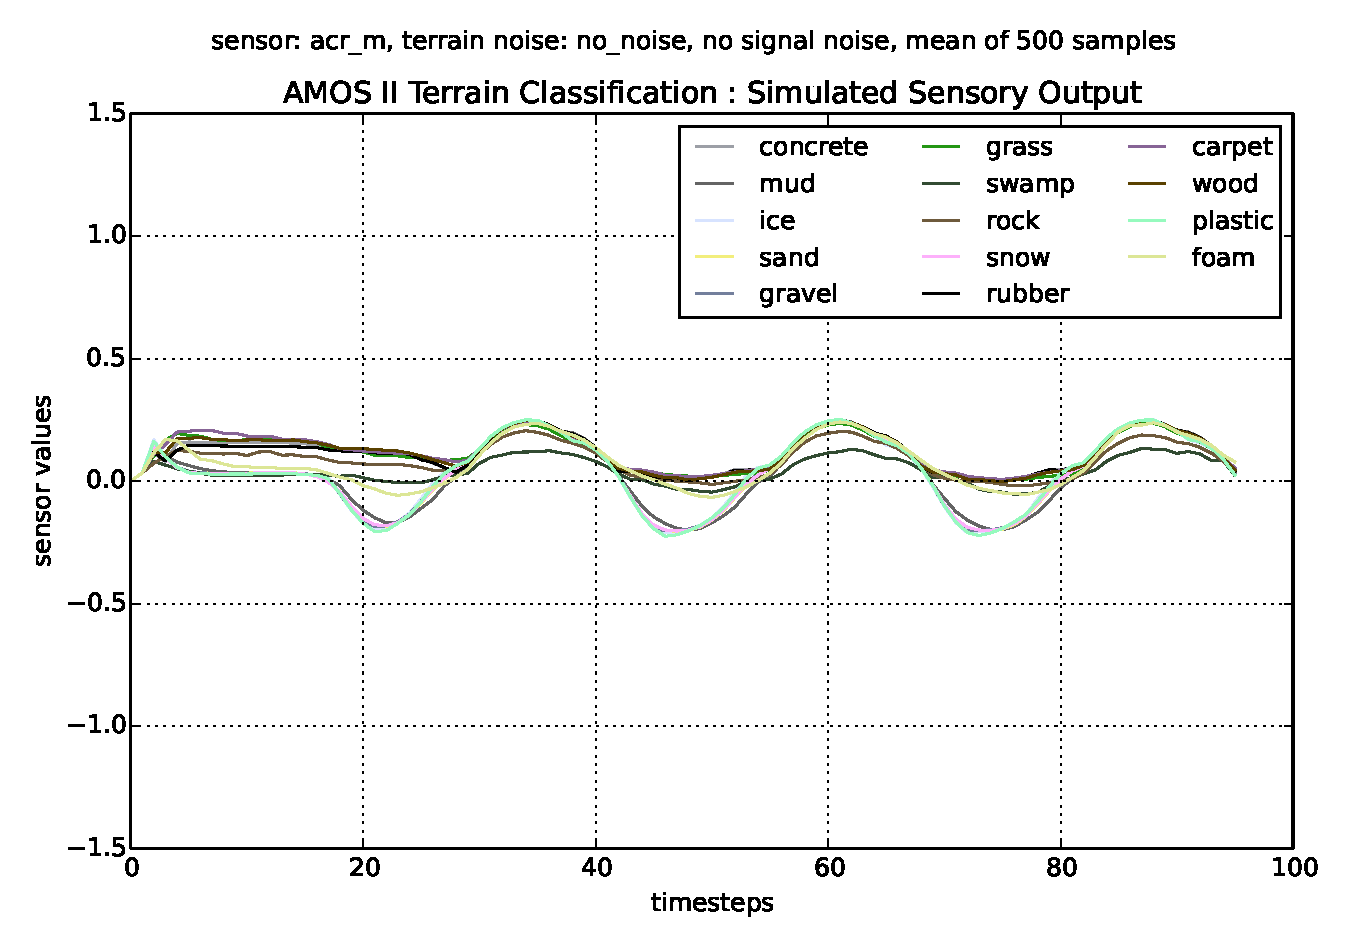
\includegraphics[width=1.0\textwidth]{sensor_acr_m_no_noise}
  \caption{Sensor ACRm : mean of 500 samples, 14 terrains}
  \label{fig:sensor_acr_m_no_noise}
\end{figure}

\begin{figure}[H]
  \centering
  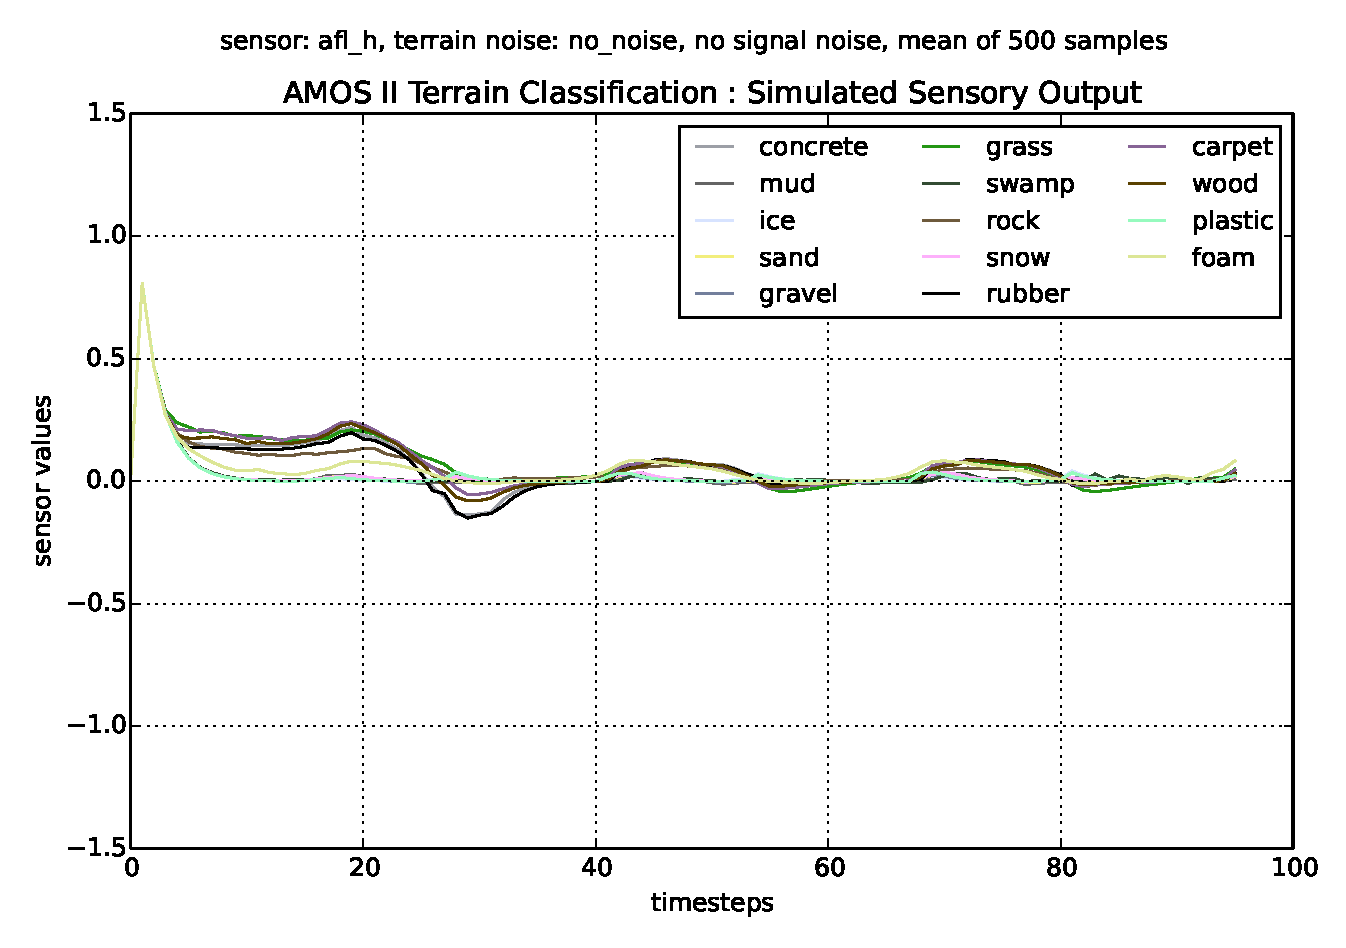
\includegraphics[width=1.0\textwidth]{sensor_afl_h_no_noise}
  \caption{Sensor AFLh : mean of 500 samples, 14 terrains}
  \label{fig:sensor_afl_h_no_noise}
\end{figure}

\begin{figure}[H]
  \centering
  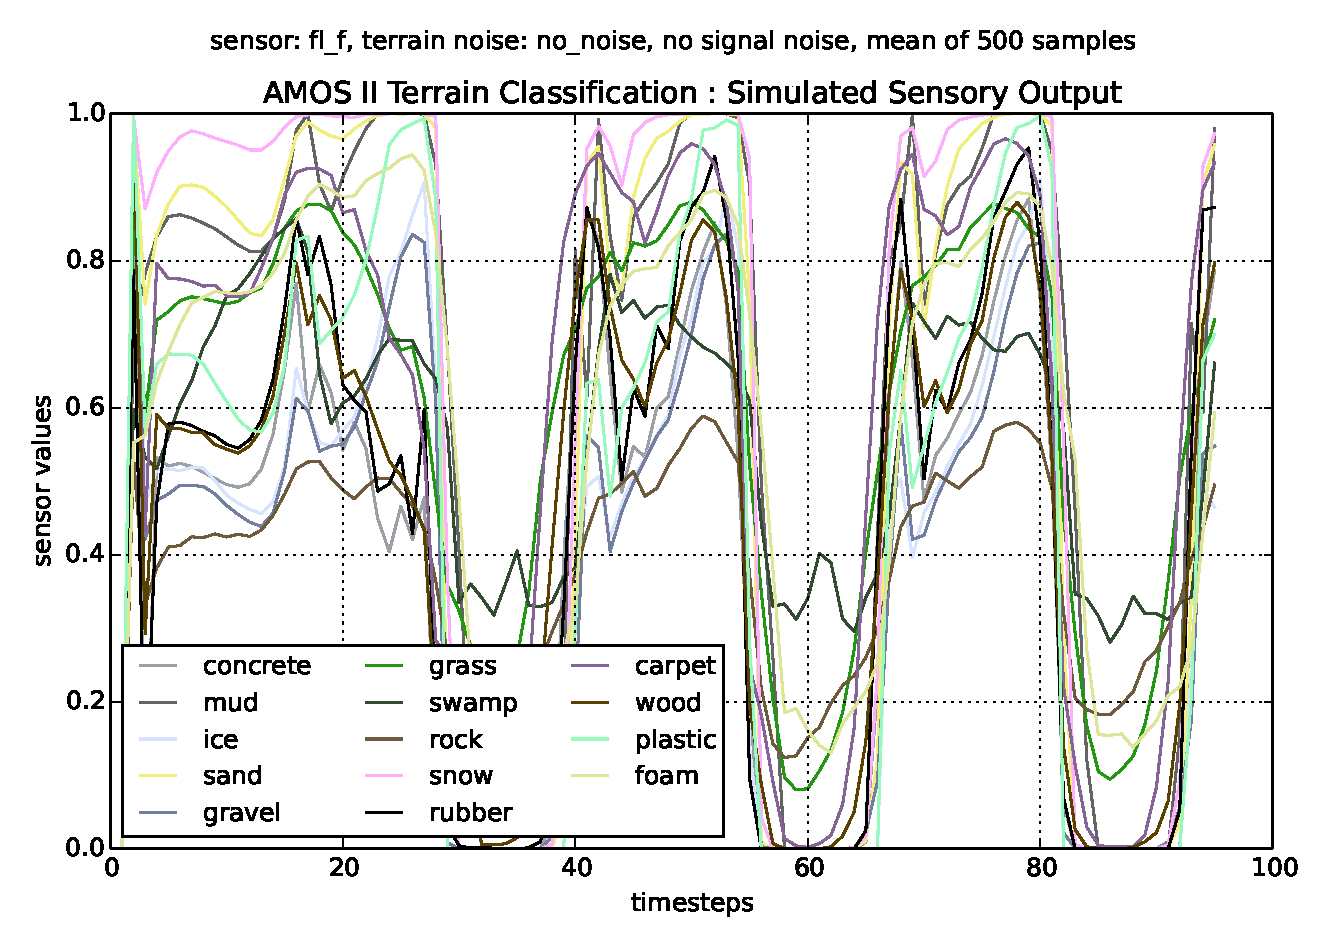
\includegraphics[width=1.0\textwidth]{sensor_fl_f_no_noise}
  \caption{Sensor FLf : mean of 500 samples, 14 terrains}
  \label{fig:sensor_fl_f_no_noise}
\end{figure}

\subsubsection*{Built Feature Vector} \label{sssec:built_feature_vectors}

\begin{figure}[H]
  \centering
  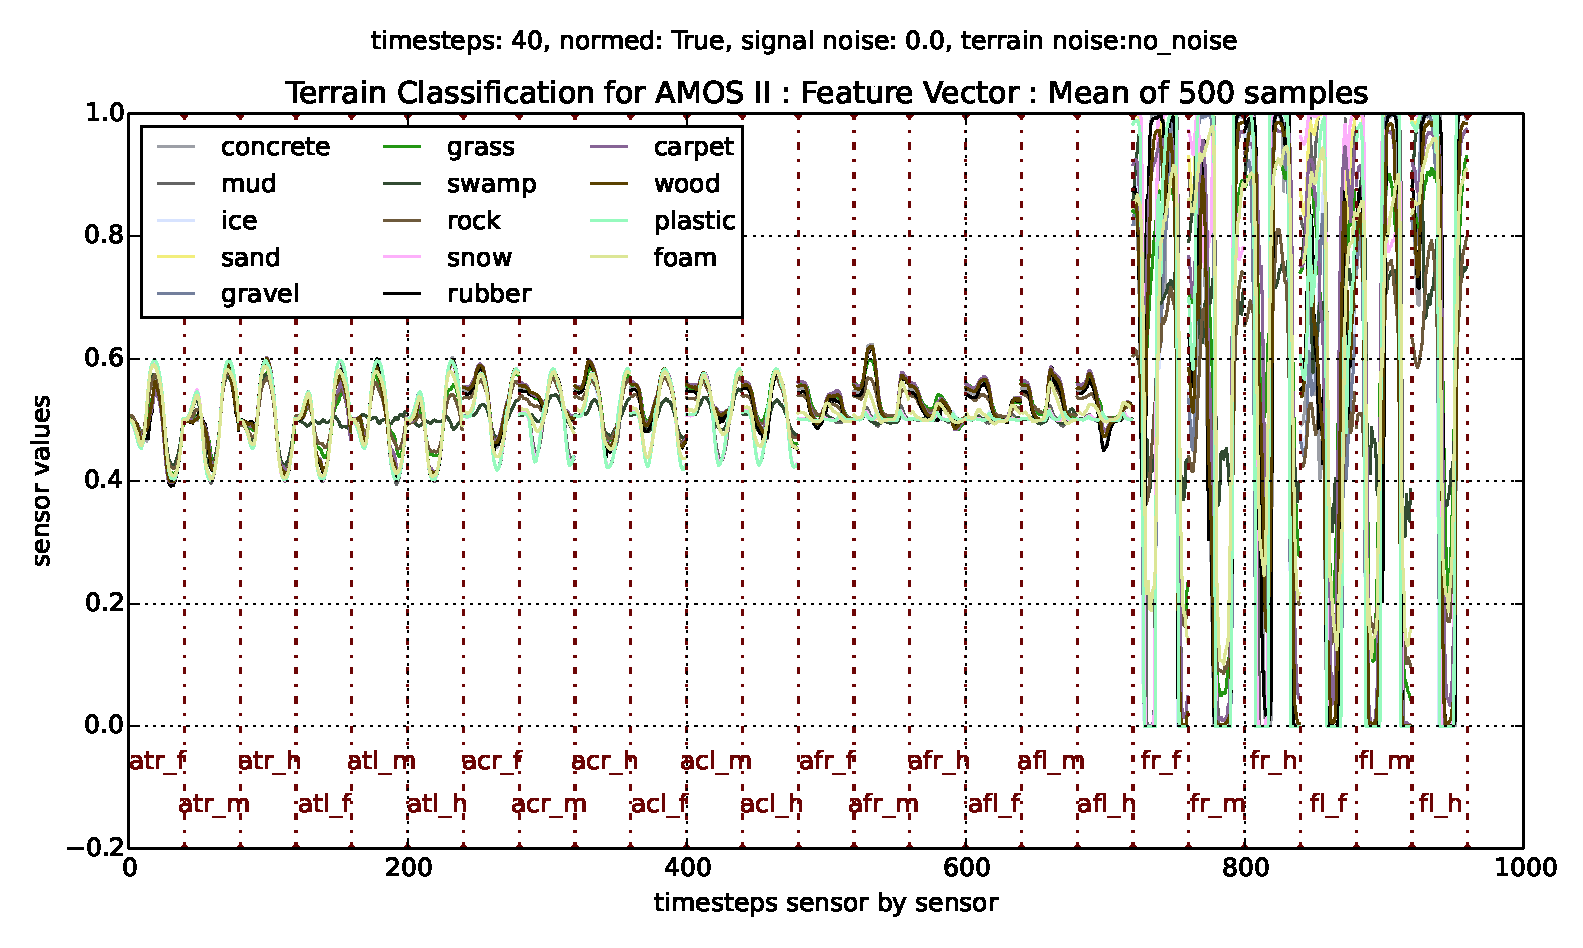
\includegraphics[width=1.0\textwidth]{sample_no_noise_0_40}
  \caption{Feature Vector : mean of 500 samples, 14 terrains, no noise, 40 timesteps}
  \label{fig:sample_40t}
\end{figure}


\begin{figure}[H]
  \centering
  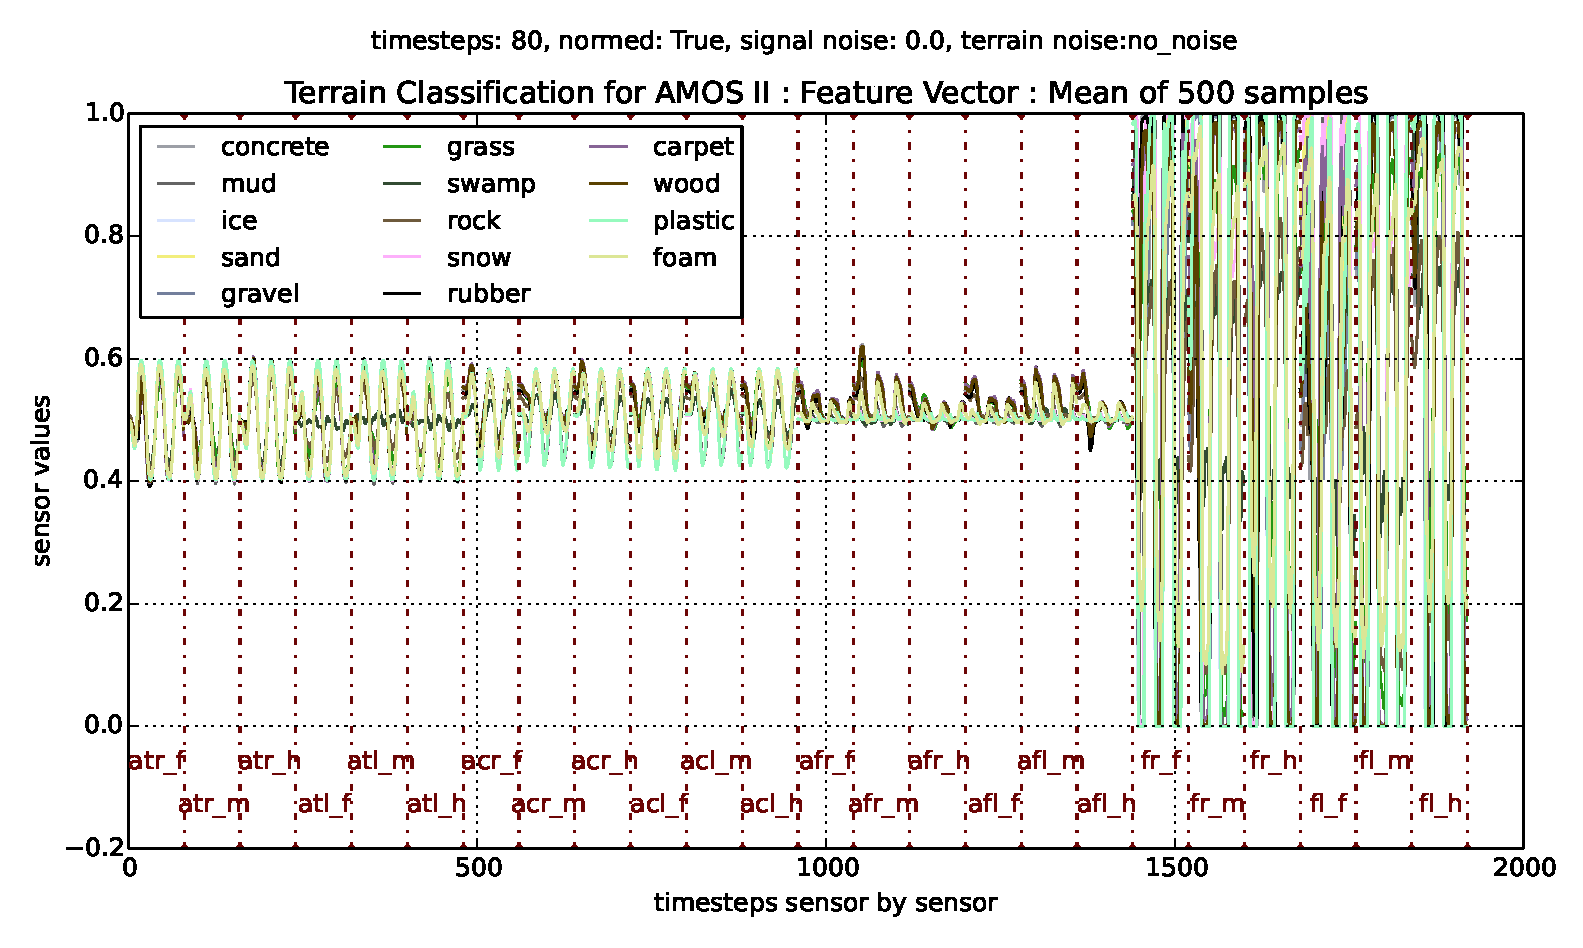
\includegraphics[width=1.0\textwidth]{sample_no_noise_0_80}
  \caption{Feature Vector : mean of 500 samples, 14 terrains, no noise, 80 timesteps}
  \label{fig:sample_80t}
\end{figure}

\subsubsection*{Terrain Noise Influence} \label{sssec:terrain_noise_influence}

\begin{figure}[H]
  \centering
  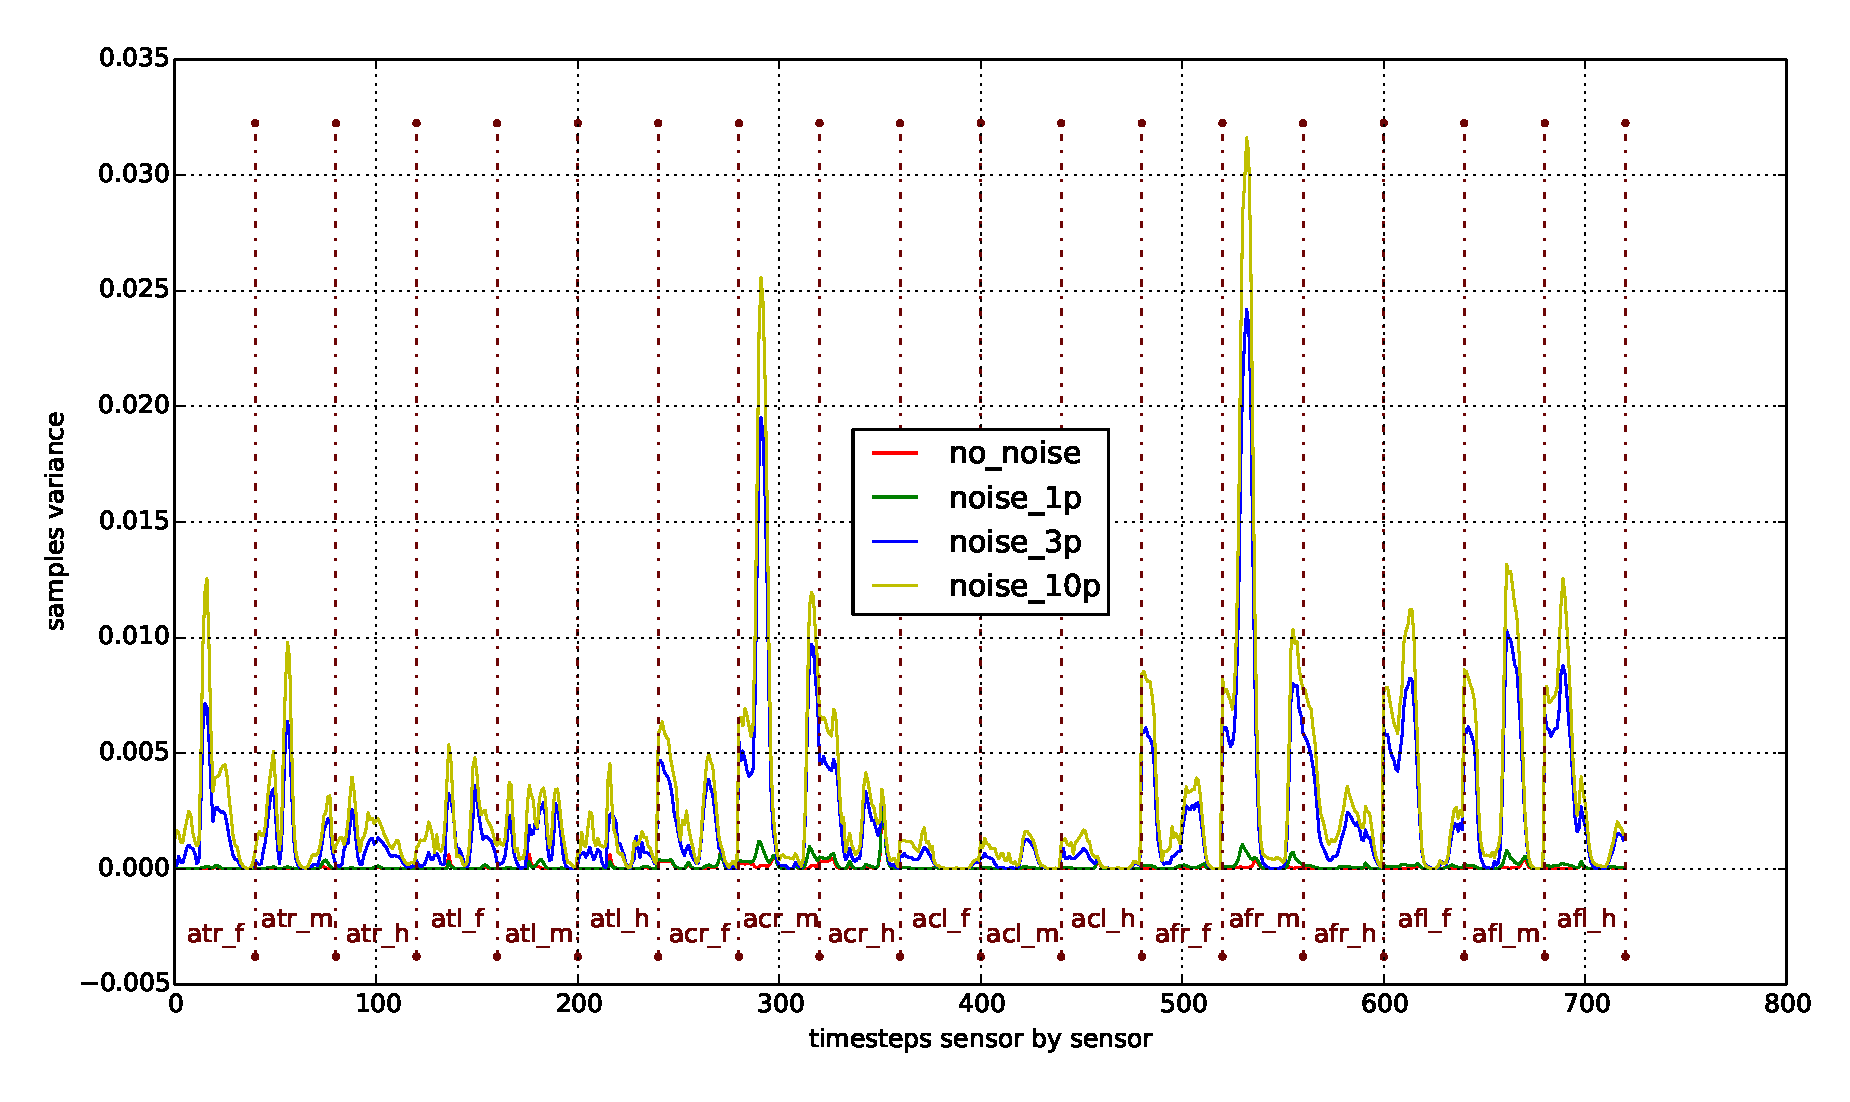
\includegraphics[width=1.0\textwidth]{tn_analysis_40_angle_gravel}
  \caption{Terrain Noise Analysis (samples variance): 500 samples, terrain gravel, angle sensors (feature vector [0:720] for 40 timesteps)}
  \label{fig:tn_analysis_angle_gravel}
\end{figure}

\begin{figure}[H]
  \centering
  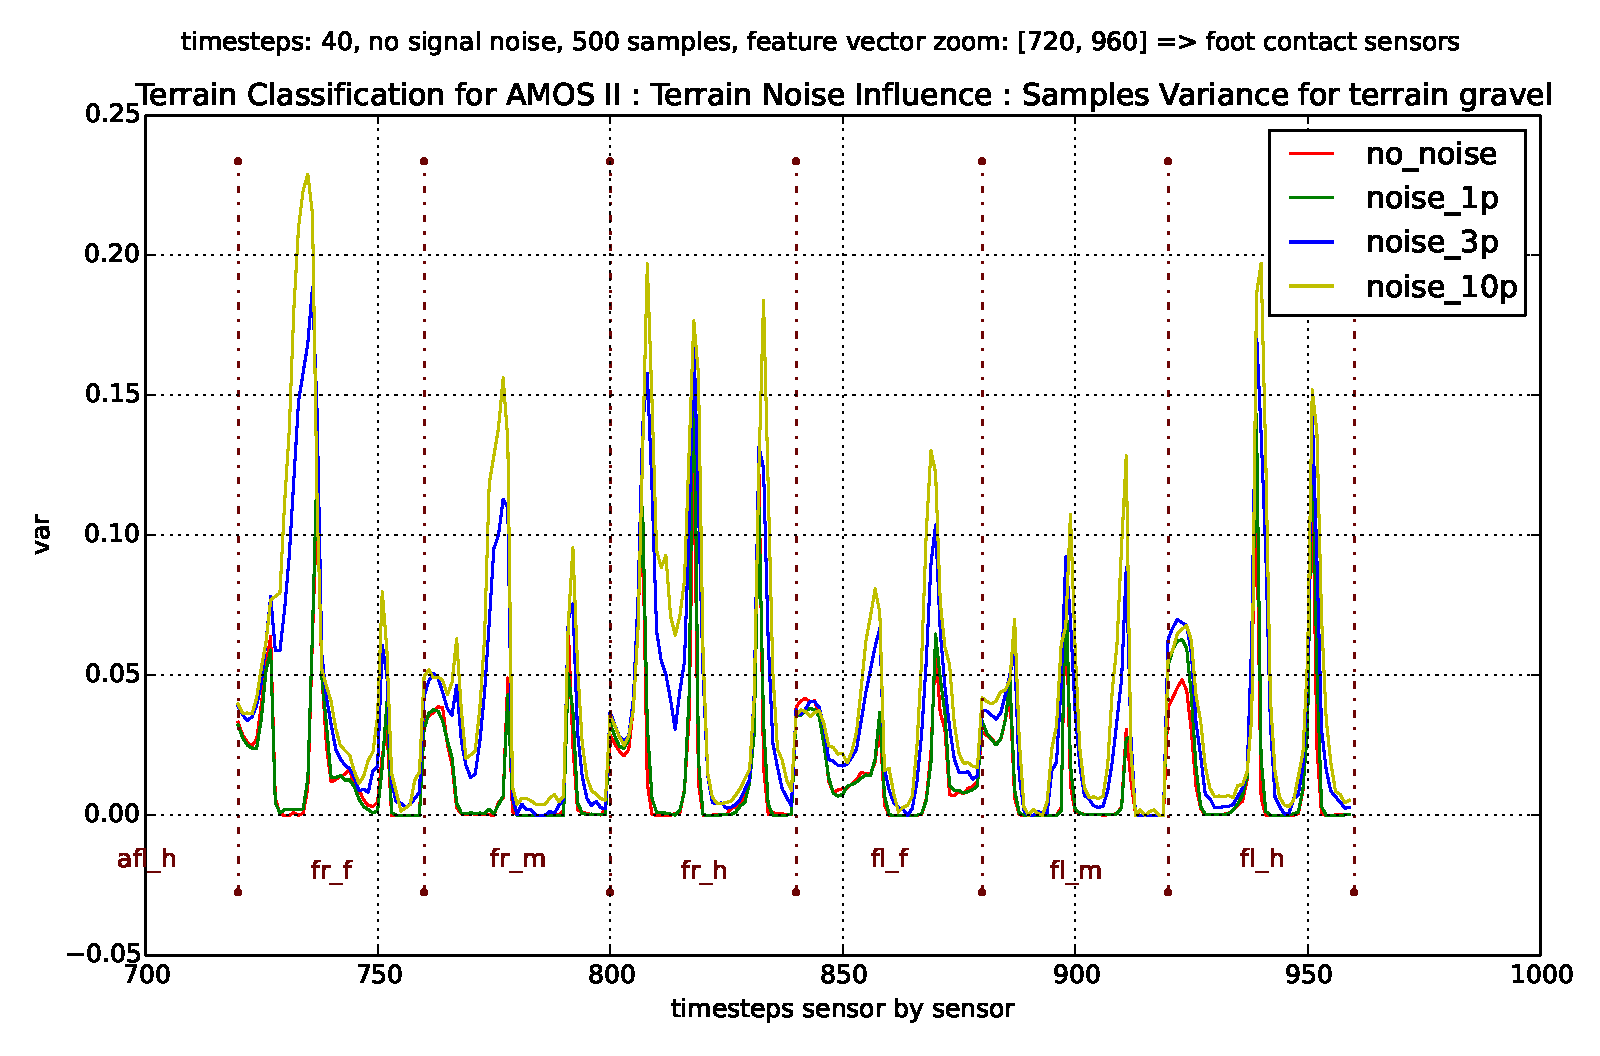
\includegraphics[width=1.0\textwidth]{tn_analysis_40_foot_contact_gravel}
  \caption{Terrain Noise Analysis (samples variance): 500 samples, terrain gravel, foot contact sensors (feature vector [720:960] for 40 timesteps)}
  \label{fig:tn_analysis_foot_contact_gravel}
\end{figure}

\begin{figure}[H]
  \centering
  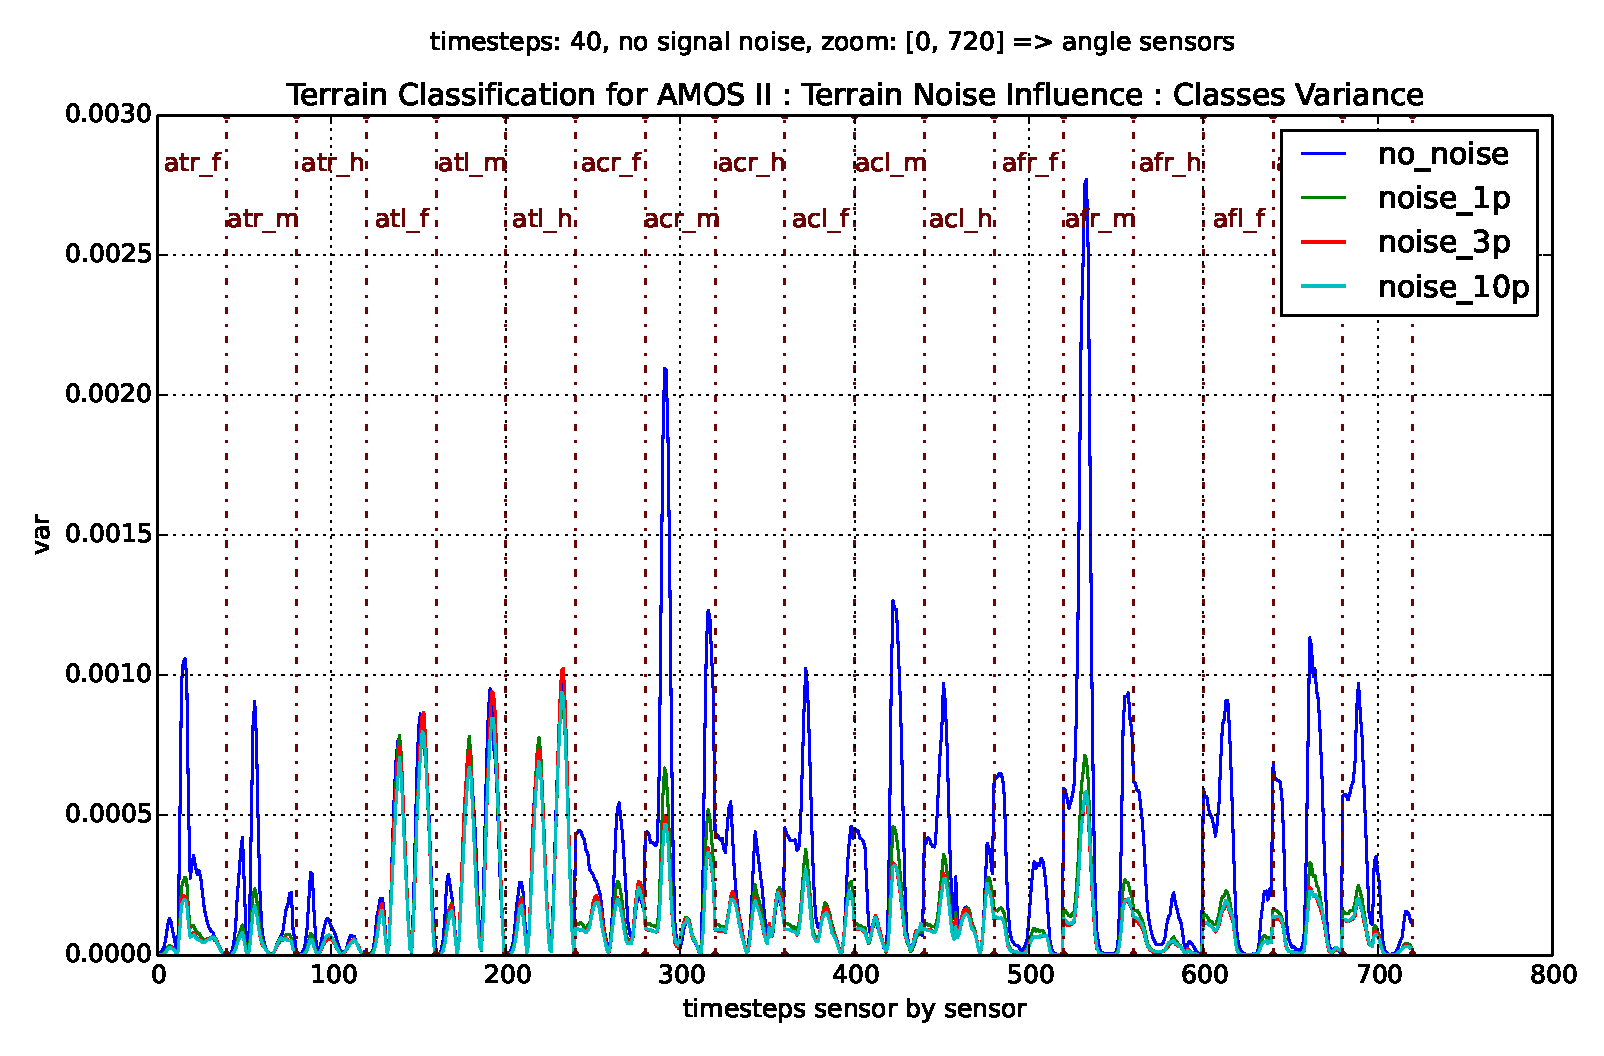
\includegraphics[width=1.0\textwidth]{tn_analysis_40_angle}
  \caption{Terrain Noise Analysis (classes variance): means of 500 samples, 14 terrains, angle sensors}
  \label{fig:tn_analysis_angle}
\end{figure}

\begin{figure}[H]
  \centering
  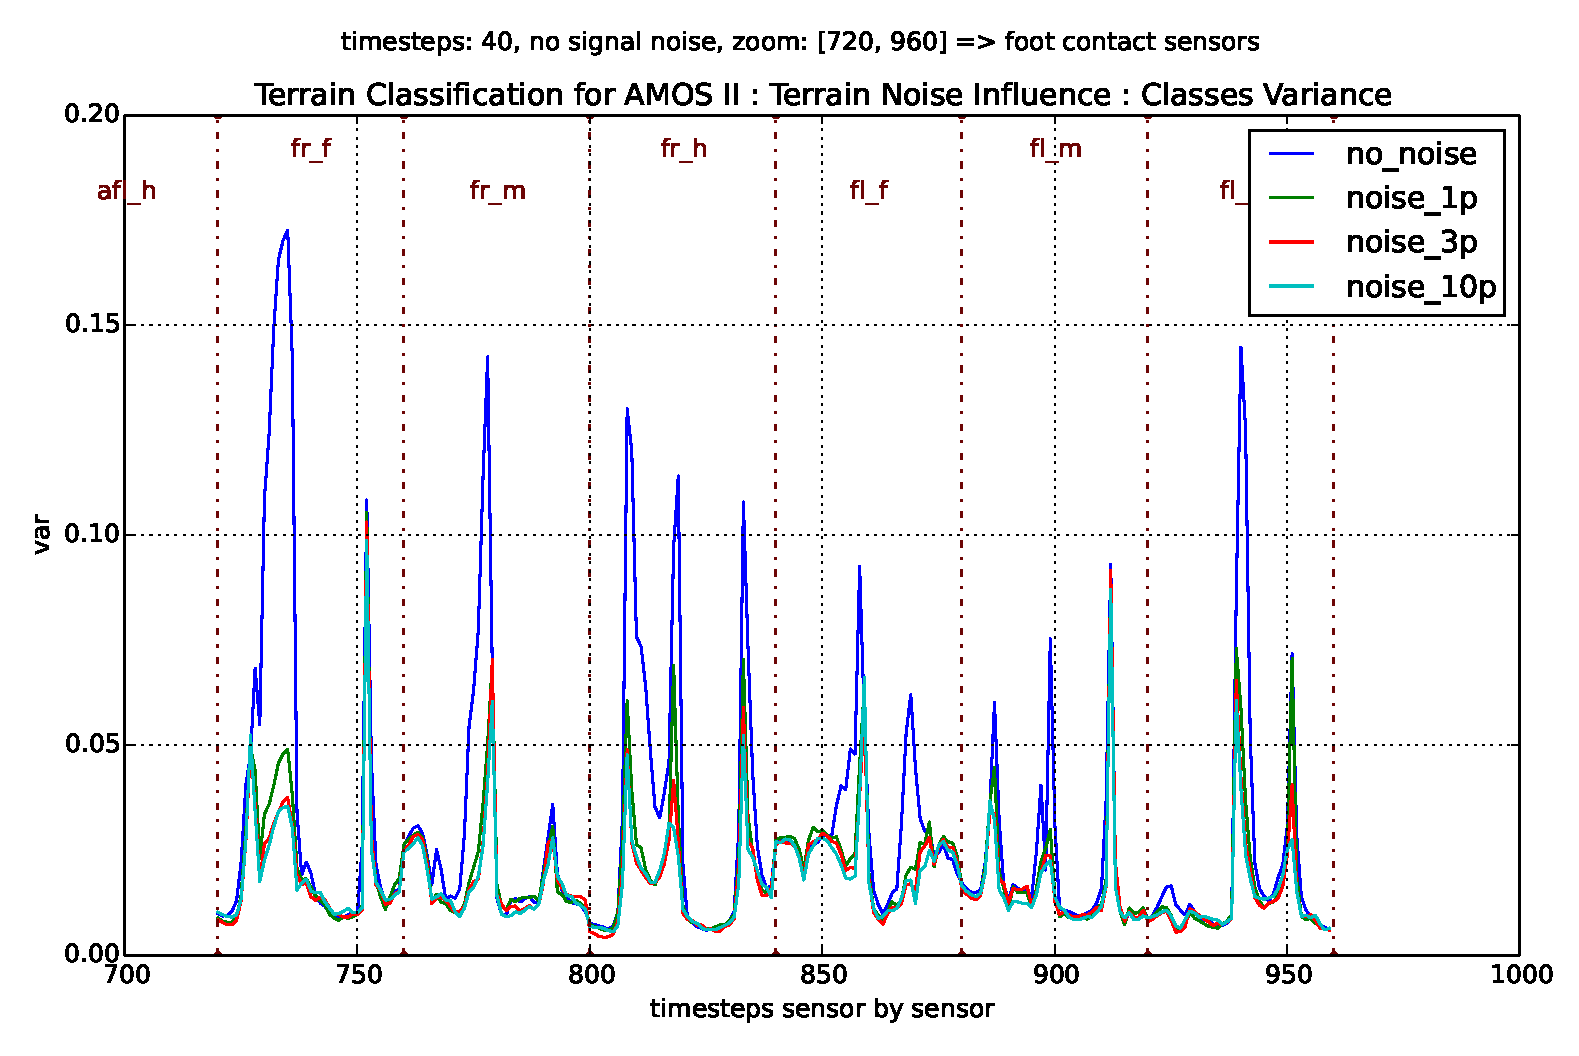
\includegraphics[width=1.0\textwidth]{tn_analysis_40_foot_contact}
  \caption{Terrain Noise Analysis (classes variance): means of 500 samples, 14 terrains, foot contact sensors}
  \label{fig:tn_analysis_foot_contact}
\end{figure}

\subsubsection*{Signal Noise Influence} \label{sssec:signal_noise_influence}


\subsection{Generated Datasets} \label{ssec:generated_datasets}

table

\subsection{Classification results} \label{ssec:classification_results}

\subsection{Final Configuration} \label{ssec:final_configuration}


evaluation (tables and figures) of classification:
\begin{itemize}
\item various terrain noise standard deviation values
\item various signal noise standard deviation values
\item various sensors on network input (only foot, only angle...)
\item various timesteps used as one sample (-> time needed for detection)
\item various number of detected terrains as outputs
\item various network structures
\item various training parameters (epochs, learning rate, batch size...)
\end{itemize}


evaluation of neural nets as a classifier:
\begin{itemize}
\item comparison to other classifiers on the same data, classifiers are ready provided by sknn library
\end{itemize}

evaluation of proprioception sensing against other methods (visual, haptic, laser...):
\begin{itemize}
\item comparison to the results from the literature
\end{itemize}

evaluation of the pruning algorithm:
\begin{itemize}
\item various starting structures, ends up with the same minimal-optimal structure?
\item various noise types, same minimal structure?
\item speed comparisons of the fully-connected vs. pruned structure
\item further analysis:
 \begin{itemize}
 \item which sensors are redundant/crucial
 \item which sensors are important for which terrain
 \item comments on the minimal structure and benefits of having it
 \end{itemize}
\end{itemize}
10-15 pages (many figures, tables)
